\listfiles
\documentclass[twoside,12pt]{article}
\newcommand{\dataset}{{\cal D}}
\newcommand{\fracpartial}[2]{\frac{\partial #1}{\partial  #2}}
\usepackage{hyperref}
\usepackage{enumerate}
\usepackage[top=2in, bottom=1.5in, left=0.85in, right=0.5in]{geometry}
\usepackage[hyphenbreaks]{breakurl}
%\usepackage[pdfstartview=FitH,pdfstartpage=13,pdfpagemode=UseNone]{hyperref}
\usepackage{amsfonts}
\usepackage{graphicx} 
\usepackage[linesnumbered,ruled]{algorithm2e}
\usepackage{float}
\usepackage{amssymb,amsmath}
\usepackage{mdwlist }
\usepackage{color}
\usepackage{multirow}
\usepackage{listings}
\usepackage{float}

\definecolor{darkblue}{rgb}{0.0,0.0,0.5}
\newtheorem{Dfn}{Definition}
\hypersetup{colorlinks,breaklinks,
            linkcolor=darkblue,urlcolor=darkblue,
            anchorcolor=darkblue,citecolor=darkblue}
\newcommand{\sign}{\text{sign}}
\newcommand{\argmin}{\arg\!\max}
\begin{document}

\title{ Conditional Random Fields for Punctuation Prediction\\  Learning Algorithms, Project 2}
\author{Mohsen Malmir, Erfan Sayyari}
\maketitle
\section{Abstract}

\section{Introduction}
In this paper, we provide the results and details of implementation of a Conditional Random Field (CRF) model for predicting English language text punctuations. CRFs are a variant of undirected graphical models that are well suited for predicting structured labels. We train our model by maximizing log conditional likelihood (LCL) of the training data. During our experiments, we found that the model could predict individual tags by more than 94\% accuracy. However, as we performed more and more experiments, we discovered the over fitting to some prevalent tags in the training set. Using several experiments and methods that will be described later in this paper, we could overcome the over-fitting problem to some degrees.\\
We choose two techniques to train the proposed model: Collin's Perceptron and Contrastive Divergence. Both of these methods are approximations to the general gradient following method. We choose these two methods because of their two characteristics: simplicity and elegance. Both Collin's Perceptron and Contrastive Divergence provides simplified updates rule for the parameters, which are less expensive compared to the general gradient following for maximizing LCL. Despite simplicity, both methods have very clear and intuitive explanation behind them: they maximize the LCL of the data by throwing spurious samples at the model. However, as we explain our experiments in more details, we do not stick to the basic algorithms and tweak them in several ways to improve their performance.\\
One of the most important parts of the CRF model for predicting text punctuation is the choice of feature functions as it effects both the performance and accuracy of the model. The feature functions we develop here use Part-of-Speech (POS) tags of the input sentence. The main characteristic for the proposed feature functions is their efficiency in computation time: training of our method only takes a few minutes on a single core machine. We show that using these feature functions, the model can predict the punctuation tags with high accuracy.\\ 
For the given training and test data, danger of over-fitting is high because of the imbalanced distribution of punctuation tags. We deal with this problem with different techniques. We show how bounding the weight parameters and early stopping can improve the accuracy for the Collin's Perceptron. By introducing random sampling and guided sampling, we achieve similar improvements in Contrastive Divergence. Then we introduce the Turn-taking train procedure: for each tag we train a different predictor and then combine them using .... We show this last technique is much more effective and achieves the highest accuracy for punctuation prediction for the given data set.


\section{Design and Analysis of Algorithm}
\subsection{The general log-linear model}
\subsection{Feature functions}
\subsubsection{Part of Speech tagging}
\subsection{Conditional random fields}
\subsection{The Collins perceptron}
\subsection{Contrastive divergence}
\subsubsection{Gibbs sampling}
\section{Design of Experiments}

To test the proposed model, we perform several experiments on the given dataset, which is an English language punctuation dataset that consists of 70115 training and 28027 test sentences. We use only training data to fit the model,  one third for validation and two thirds for training.	 After training is complete, the test data is used to assess prediction and generalization of the model. Each sentence in the training data consists of a set of words without any punctuation symbols. For multiple sentences, there was a few form of syntax complications such as use of '\$' in place of the word 'money', or words that were split to two parts by space *****. We ignored all such cases, as they were few sentences and finding a complete list of them required going through the entire dataset which was very time consuming.\\


\subsection{Initialization}
For Collin's Perceptron, as pointed out in the lecture, the learning rate can be fixed to $\lambda=1$. This is because scaling scaling the weight vector $w$ does not affect the predicted label by the model. Using different learning rates leads to different weight vectors that are scaled versions of each other. However, one should note that this is correct only if the model converges to the global optimum ******. For both experiments on Collin's Perceptron and Contrastive Divergence, we fix $\lambda \leftarrow 1$. \\
For initializing the weight vector $w$, we use small random Normal numbers from $\mathcal N(0.,1e-5)$. This is because as we describe later, limiting the weight vector entries $w_j$ to be in a small range $[-a,a]$ helps to prevent over-fitting. Because both $a$ and $-a$ represents the extreme learned situation, a good option for initial weights is a random vector that is not biased for specific feature functions, that is $w_j$ better be close to 0 for all $j$.\\
\subsection{Preprocessing}
\subsection{Performance Measure}
We report the performance of the models in two different ways. First, we report the prediction of individual target tags, That is, how accurate the model can predict the individual punctuations tags in corpus sentences. We report the accuracy of prediction for the entire tags as wells as individual target tags. The benefit of looking into individual punctuation tag prediction is that it reveals if over-fitting has happened due to imbalanced distribution of tags in the training data. Next, we report the accuracy of model for predicting sentence punctuation. The accuracy for this case should be lower because each sentence punctuation is composed of multiple tags. 
\section{Results of Experiments}
\subsection{Collins perceptron}
For training Collin's Perceptron, we divide the training data into two thirds for training and one third for validation. The initial value for the weight vector entries $w_j$ is chosen to be small random numbers from $\mathcal{N}(0,1e-5)$. We use early stopping as a criteria for terminating the training procedure. Because Collin's Perceptron has no hyper parameters, there is a chance of over fitting to the training data. In the train procedure, we divide the data into train and validation sets and start training only with train data. After each epoch, we measure the accuracy for predicting individual punctuation tags on the validation data. If the accuracy has decreased, we stop the training and roll back the weights to previous values.\\
For the first experiment, we train Collin's perceptron with early stopping. Figure \ref{figEarlyStoppingPercGibbs} shows that the training stops after 4 epochs. However, after the first epoch, the model is almost converged and the accuracy changes a small amount after that. The accuracy for predicting individual tags and sentences for validation and test sets are shown in Table \ref{tablePredPerceptron}.\\

\begin{figure}[H]
\centering
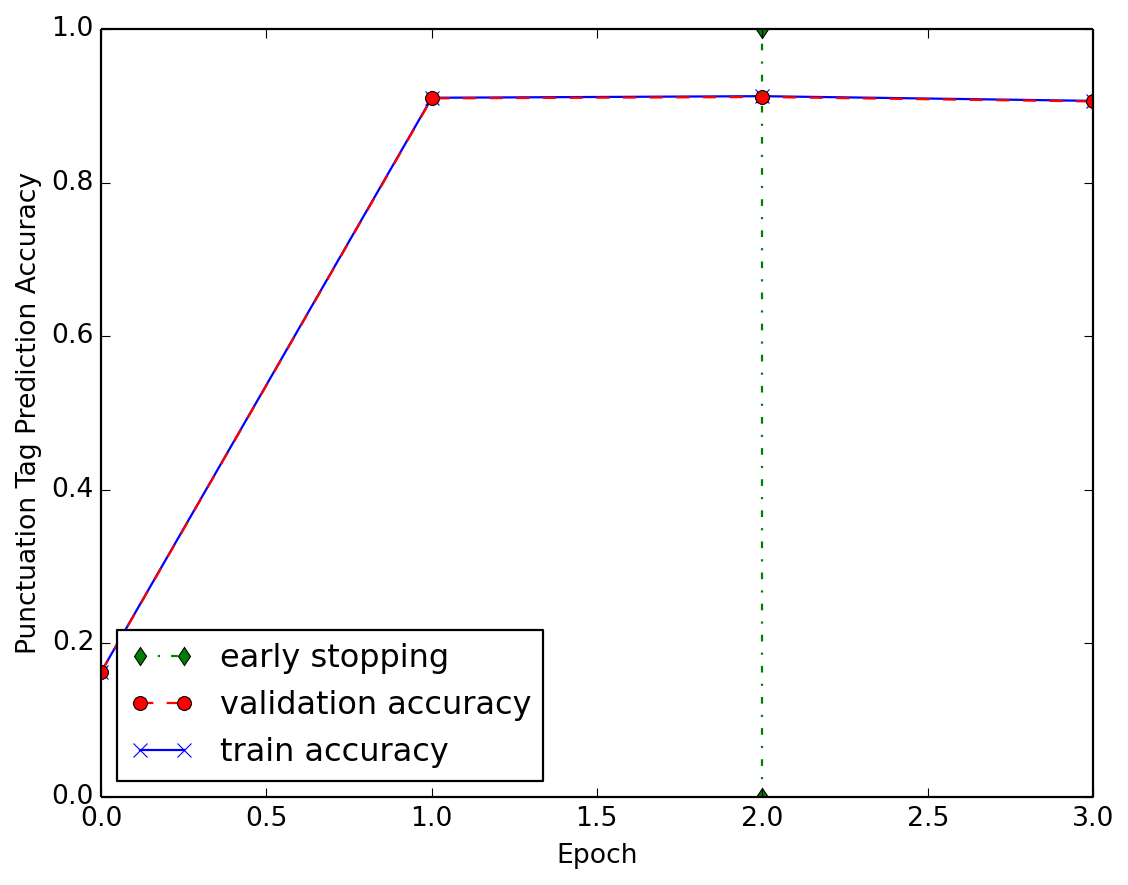
\includegraphics[width=.7\textwidth]{./figs/Perceptron/Perceptron.png}
\caption{Early stopping for Collin's Perceptron. }
\label{figEarlyStoppingPercGibbs}
\end{figure}

\begin{table}[H]\footnotesize
  \caption{Collin's Perceptron performance on the given data set}
\begin{center}
    \begin{tabular}{| c | c | c | }
    \hline
    \textbf{ Measure} & \textbf{Validation set accuracy} & \textbf{Test set accuracy} \\ \hline
    Individual tag prediction & 0.911 & 0.901  \\ \hline
    Sentence level prediction & 0.389 & 0.371  \\ \hline
    \end{tabular}
    \label{tablePredPerceptron}
\end{center}
\end{table}


In order to further assess the correctness of the model, we look into the accuracy for predicting individual tags, that is, how much the model is accurate in predicting different punctuation tags. Table \ref{tableIndividualTagsPerceptron} shows the accuracy for predicting individual tags. Figure \ref{figPerceptronConfMat} shows the confusion matrix for the same prediction problem. A quick look at table \ref{tableIndividualTagsPerceptron} and figure \ref{figPerceptronConfMat} reveals some properties of the Collin's Perceptron model. Here, the model has learned only the most frequent punctuation tags in sentences, that is SPACE and PERIOD. For each test sentence the model predicts a simple punctuation tag sequence which has SPACE or PERIOD in most positions (look at SPACE and PERIOD columns in the test confusion matrix in figure \ref{figPerceptronConfMat}). This behavior is somehow natural, because in training phase, the model sees sequences of tags with SPACE or PERIOD more often, and thus the corresponding weights to these weights are more frequently updated. Table \ref{tablePerceptronWeights} shows 5 largest entries in the weight vector and their corresponding feature function (******* DESC FOR FFs).

\begin{table}[H]\footnotesize
  \caption{Accuracy of predicting different tags by Collin's Perceptron}
\begin{center}
    \begin{tabular}{| c | c | c | c | c |}
    \hline
    \textbf{ Method} & \multicolumn{2}{ c| }{\textbf{Validation set}}  & \multicolumn{2}{ c| }{\textbf{Test set}} \\ \hline
     & Accuracy & Frequency & Accuracy & Frequency \\ \hline
    EXCLAMATION\_POINT & 0.0 & 2567 & 0.0 & 1066  \\ \hline
    SPACE & 0.947 & 580077  & 0.947 & 235536\\ \hline
    QUESTION\_MARK & 0.145 & 10904 & 0.1444 & 4792 \\ \hline
    PERIOD & 0.849 & 57259  & 0.847 & 22492\\ \hline
    COLON & 0.009 & 1009  & 0.003 & 1174\\ \hline
    COMMA & 0.248 & 28555  & 0.262 & 10665\\ \hline
    \end{tabular}
    \label{tableIndividualTagsPerceptron}
\end{center}
\end{table}

\begin{figure}[H]
\centering
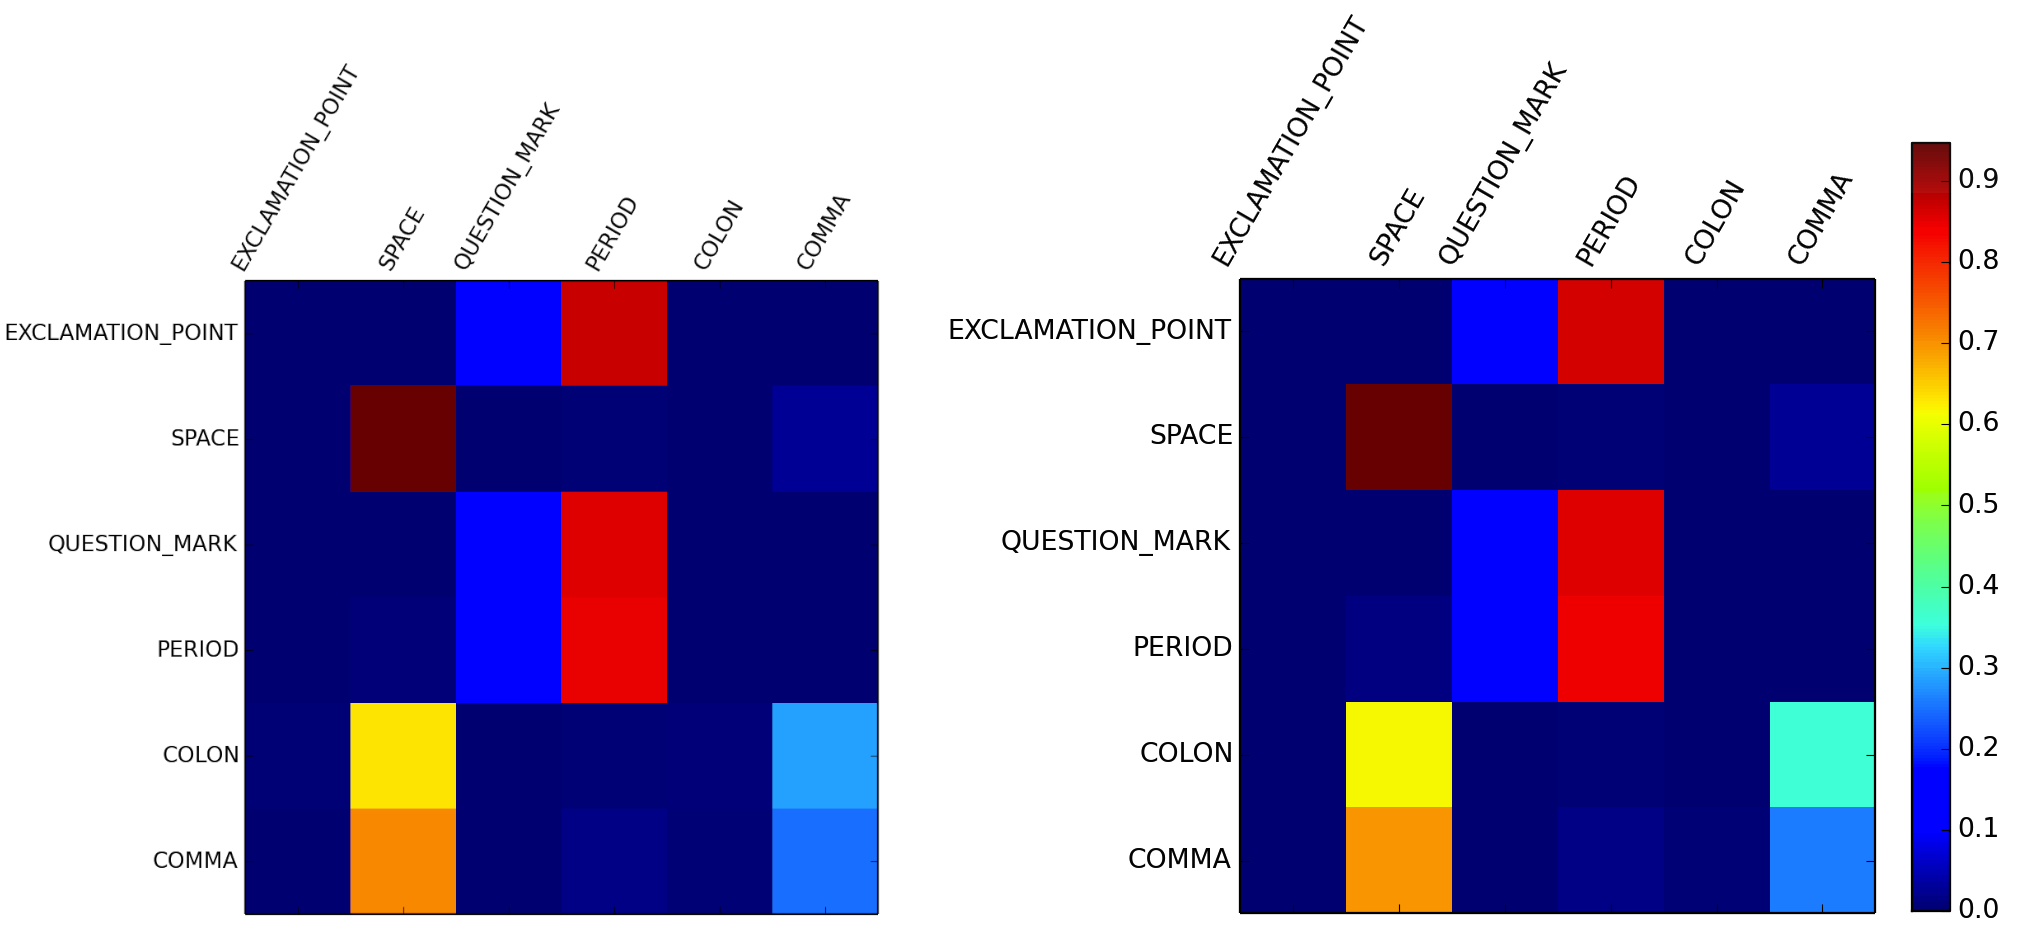
\includegraphics[width=1.\textwidth]{./figs/figPerceptronConfMat.png}
\caption{Confusion matrix for predicting individual tags using Collin's Perceptron on Left: validation, and Right: test sets.}
\label{figPerceptronConfMat}
\end{figure}


\begin{table}[H]\footnotesize
  \caption{20 Largest entries of the weight vector  for Collin's Perceptron after learning. For each weight entry, its magnitude and corresponding feature function is listed.}
\begin{center}
    \begin{tabular}{| c | c | c | c | c |}
    \hline
    \textbf{ Magnitue} & $X_{i-1}$ & $X_i$ & $Y_{i-1}$& $Y_i$ \\ \hline
3964.99 & NN & VB & COMMA & SPACE  \\ \hline
3927.99 & NN & VB & SPACE & SPACE  \\ \hline
3308.99 & ADJ & NN & SPACE & COMMA  \\ \hline
2875.99 & IN & NN & SPACE & COMMA  \\ \hline
2460.99 & PRP & NN & SPACE & COMMA  \\ \hline
2099.00 & NN & IN  & COMMA & SPACE  \\ \hline
2067.00 & NN & IN & SPACE & SPACE  \\ \hline
1800.99 & NN & NN & COMMA & SPACE  \\ \hline
1771.99 & PRP & VB & SPACE & COMMA  \\ \hline
1759.00 & NN & NN & SPACE & SPACE  \\ \hline
1508.99 & NN & WRB & COMMA & SPACE  \\ \hline
1463.00 & NN & WRB & SPACE & SPACE  \\ \hline
1451.00 & NN & PRP & COMMA & SPACE  \\ \hline
1409.00 & NN & PRP & SPACE & SPACE  \\ \hline
1209.99 & ADJ & PRP & COMMA & SPACE  \\ \hline
1198.99 & VB & ADJ & SPACE & COMMA  \\ \hline
1077.00 & ADJ & PRP & SPACE & SPACE  \\ \hline
1056.00 & NN & ADJ & COMMA & SPACE  \\ \hline
1018.99 & NN & ADJ & SPACE & SPACE  \\ \hline
997.000 & IN & PRP & SPACE & COMMA  \\ \hline
    \end{tabular}
    \label{tablePerceptronWeights}
\end{center}
\end{table}

\subsection{Contrastive Divergence}
For Contrastive Divergence, the training setup is the same as mentioned in previous section. The training data is divided into training and validation sets, and early stopping is applied to terminate the training. The initial value for the weight vector entries are chosen randomly from $\mathcal{N}(0,1e-5)$. 
\subsubsection{Training with Bounded Weights}
As we saw in Collin's Perceptron, the weight vector entries grow unbounded for tags that are more frequent in the training data. This unbounded growth can cause problems during prediction, because the large weights tend to bias the decision in favor of more frequent tags (e.g. SPACE or PERIOD). One way to deal with this situation is to use a separate learning rate for each entry in the weight vector. Then if a $w_j$ has been updated frequently, we can decrease its learning rate. A  similar approach is to force the $w_j$s to be in a specified range $[-a,a]$. For each update, one then should check that $w_j$ doesn't exceed this bound. We adapt this technique in training of Contrastive Divergence model, with hope that this reduces over-fitting to specific punctuation tags.\\
Figure \ref{figCDEarlyStopping} shows that early stopping terminates the training for Contrastive Divergence after two epochs. Tables \ref{tablePredGibbs} and \ref{tableIndividualTagsGibbs} show the performance for this model. These results are very interesting as we compare it row by row to table \ref{tableIndividualTagsPerceptron}. We see that the tag EXCLAMATION\_POINT, QUESTION\_MARK and COLON are learned more and accuracy of their prediction has  increased in Contrastive Divergence compared to Collin's Perceptron. Specifically this is interesting because these are the lowest frequency symbols in the training dataset. However, this learning occurred at the expense of \emph{unlearning} COMMA and PERIOD, which lead to decreased overall prediction accuracy both on sentence level and individual tag level prediction.  Table \ref{tableGibbsWeights} displays some of the weights learned by Contrastive Divergence. (*****DESC FOR FFs)

\begin{figure}[H]
\centering
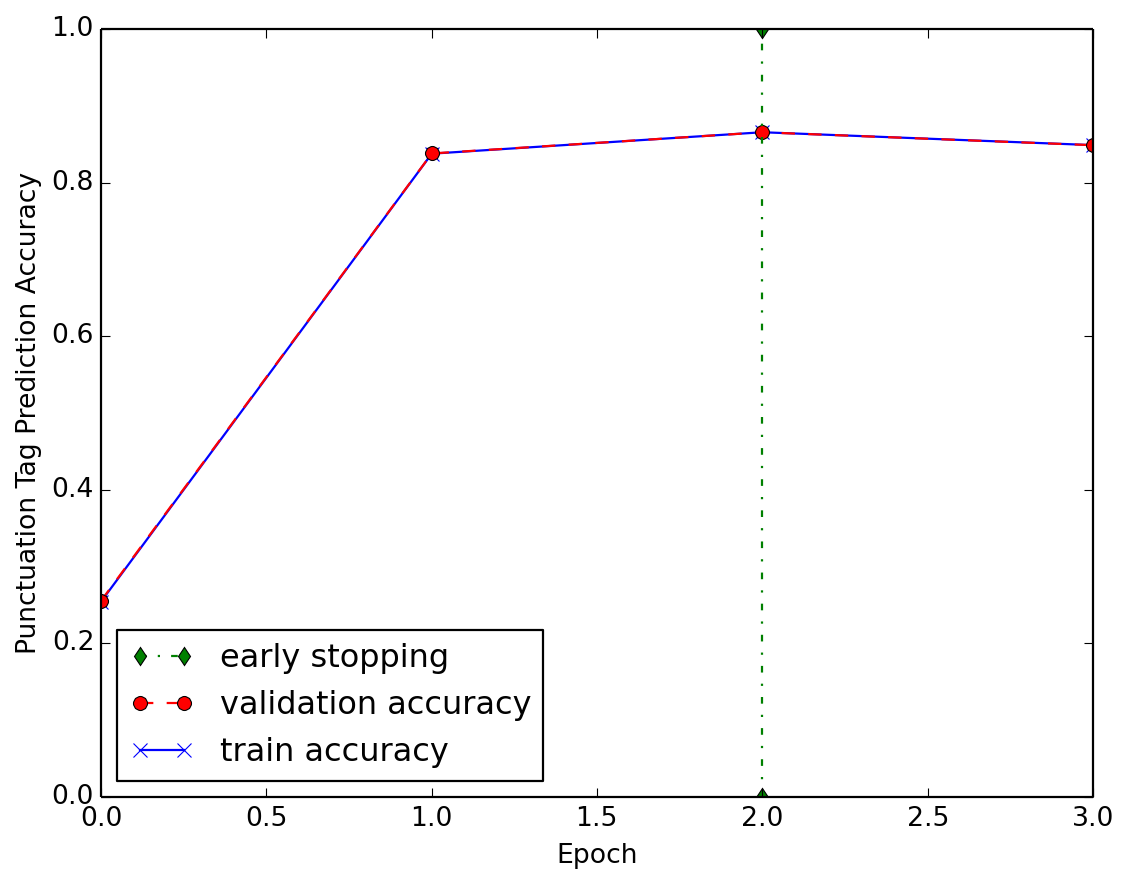
\includegraphics[width=1.\textwidth]{./figs/Gibbs/CD.png}
\caption{Early stopping for Contrastive Divergence.}
\label{figCDEarlyStopping}
\end{figure}


\begin{table}[H]\footnotesize
  \caption{Contrastive Divergence performance on individual tag and sentence punctuation prediction.}
\begin{center}
    \begin{tabular}{| c | c | c | }
    \hline
    \textbf{ Measure} & \textbf{Validation set accuracy} & \textbf{Test set accuracy} \\ \hline
    Individual tag prediction & 0.866 & 0.852  \\ \hline
    Sentence level prediction & 0.113 & 0.115  \\ \hline
    \end{tabular}
    \label{tablePredGibbs}
\end{center}
\end{table}


\begin{table}[H]\footnotesize
  \caption{Accuracy of predicting different tags by Collin's Perceptron}
\begin{center}
    \begin{tabular}{| c | c | c | c | c |}
    \hline
    \textbf{ Method} & \multicolumn{2}{ c| }{\textbf{Validation set}}  & \multicolumn{2}{ c| }{\textbf{Test set}} \\ \hline
     & Accuracy & Frequency & Accuracy & Frequency \\ \hline
    EXCLAMATION\_POINT & 0.486 & 2567 & 0.518 & 1066  \\ \hline
    SPACE & 0.945 & 580077  & 0.947 & 235536\\ \hline
    QUESTION\_MARK & 0.249 & 10904 & 0.247 & 4792 \\ \hline
    PERIOD & 0.849 & 57259  & 0.847 & 22492\\ \hline
    COLON & 0.3 & 1009  & 0.5 & 1174\\ \hline
    COMMA & 0.086 & 28555  & 0.076 & 10665\\ \hline
    \end{tabular}
    \label{tableIndividualTagsGibbs}
\end{center}
\end{table}

\begin{table}[H]\footnotesize
  \caption{20 Largest entries of the weight vector  for Contrastive Divergence after learning.}
\begin{center}
    \begin{tabular}{| c | c | c | c | c |}
    \hline
    \textbf{ Magnitue} & $X_{i-1}$ & $X_i$ & $Y_{i-1}$& $Y_i$ \\ \hline
0.1& WRB& IN &SPACE& SPACE\\ \hline
0.1& NN &UH &SPACE &COLON\\ \hline
0.1& NN &UH &SPACE &PERIOD\\ \hline
0.1 &ADJ &WH &SPACE &SPACE\\ \hline
0.1 &PRP &ADJ &COMMA& SPACE\\ \hline
0.1 &PRP &ADJ &SPACE &QUESTION\_MARK\\ \hline
0.1 &PRP& ADJ &SPACE &SPACE\\ \hline
0.1 &IN &VB &SPACE &SPACE\\ \hline
0.1 &VB &IN &SPACE &SPACE\\ \hline
0.1 &VB &IN &SPACE &PERIOD\\ \hline
0.1 &VB &IN &SPACE &COMMA\\ \hline
0.1 &IN &VB &SPACE &QUESTION\_MARK\\ \hline
0.1 &IN &VB &SPACE &PERIOD\\ \hline
0.1 &NN &SYM &COMMA& SPACE\\ \hline
0.1 &CC &CD &SPACE &PERIOD\\ \hline
0.1 &CC &CD &SPACE &SPACE\\ \hline
0.1 &PRP &CD& SPACE &PERIOD\\ \hline
0.1 &PRP &CD &SPACE &QUESTION\_MARK\\ \hline
0.1 &PRP &EX &SPACE &QUESTION\_MARK\\ \hline
0.1 &PRP& EX &SPACE &PERIOD\\ \hline
    \end{tabular}
    \label{tableGibbsWeights}
\end{center}
\end{table}



\section{Findings and Lessons Learned}
\subsection{Numerical Issues and Preprocessing}
\subsection{Overfitting}
\subsection{Model Selection}
\subsection{Future works}
\end{document}